%\modeCorrection

%%%% début de la page
\renewcommand{\thesection}{\textcolor{red}{Partie \Roman{section} -}}
\renewcommand{\thesubsection}{\textcolor{red}{\Roman{section}.\arabic{subsection}}}
\renewcommand{\thesubsubsection}{\textcolor{red}{\Roman{section}.\arabic{subsection}.\alph{subsubsection}}}

\setcounter{section}{0}
\setcounter{document}{0}
\sndEnTeteTPOnze

\begin{center}
\begin{mdframed}[style=titr, leftmargin=60pt, rightmargin=60pt, innertopmargin=7pt, innerbottommargin=7pt, innerrightmargin=8pt, innerleftmargin=8pt]

\begin{center}
\large{\textbf{TP 12 : \'{E}tude des composés ioniques
}}
\end{center}
\end{mdframed}
\end{center}


%%%% objectifs
\begin{tcolorbox}[colback=blue!5!white,colframe=blue!75!black,title=Objectifs de la séance :]
\begin{itemize}
    \item Mettre en œuvre des tests chimiques pour identifier des ions en solution  ;
    \item Exploiter l’électroneutralité de la matière pour associer des espèces ioniques et déterminer la formule d’un composé ionique ;
\end{itemize}
\end{tcolorbox}

%%%% Consignes
\begin{tcolorbox}[colback=red!5!white,colframe=red!75!black,title= Consignes :]
\begin{itemize}
    \item Faire attention au matériel lors de son utilisation ;
\end{itemize}
\end{tcolorbox}

%%%% contexte
\section{Analyse documentaire}
\begin{tcolorbox}[colback=orange!5!white,colframe=orange!75!black,title= Contexte : à quoi sert le nigari ? :]

\begin{minipage}{0.75\textwidth}
    Vous avez retrouvé dans votre cuisine un pot de nigari, un solide ionique naturel commercialisé sous forme de paillettes. Vous vous rappelez que ce nigari vous avez été recommandé pour les effets positifs qu'il pourrait avoir sur votre corps. Malheureusement, une partie de l’étiquette du pot de nigari s’est effacée et vous ne savez plus exactement pourquoi il vous avait été recommandé. 
\end{minipage}
\begin{minipage}{0.2\textwidth}
\begin{center}
    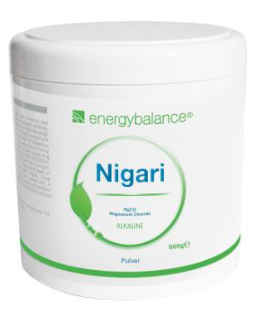
\includegraphics[scale=0.7]{Images/Nigari.PNG}
\end{center}
    
\end{minipage}

\problematique{Comment retrouver les bienfaits du nigari pour la santé ?}
\end{tcolorbox}


\begin{mdframed}[style=autreexo]
\textbf{\bsc{Liste du matériel}}
\vspace{-0.5cm}
\begin{multicols}{2}
\begin{itemize}
    \item Des paillettes de nigari ;
    \item Une solution d'oxalate d'ammonium ;
    \item Une solution d'hydroxyde de sodium ;
    \item Une solution de nitrate d'argent ;
    \item Une pissette d'eau distillée ; 
    \item Une spatule ;
    \item Des tubes à essais ;
\end{itemize}
\end{multicols}
\end{mdframed}
\clearpage

%%%% documents
\begin{doc}{Applications de quelques ions}
\vspace{-0.8cm}
\begin{center}
    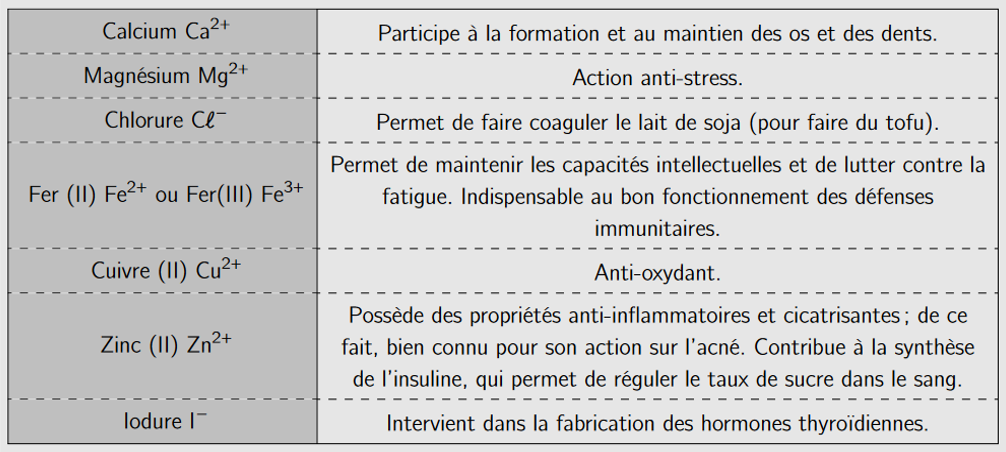
\includegraphics[scale=0.73]{Images/Ions.png}
\end{center}
\end{doc}

\begin{doc}{Identification de quelques ions}
\vspace{-0.8cm}
\begin{center}
    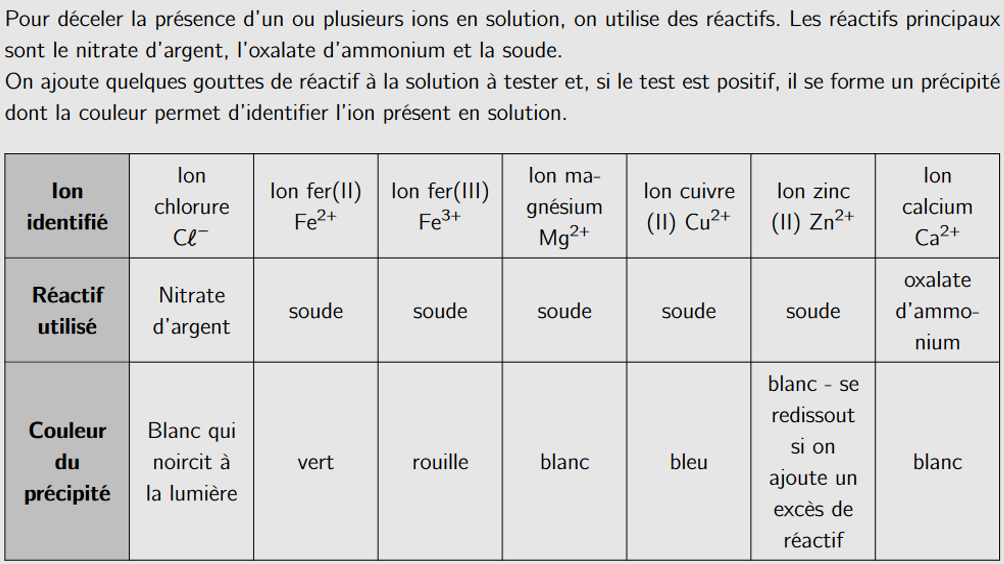
\includegraphics[scale=1]{Images/Ions_identification.png}
\end{center}
\end{doc}
\newpage
\begin{doc}{Définition et propriété d'un composé}
\vspace{-1cm}
\begin{center}
    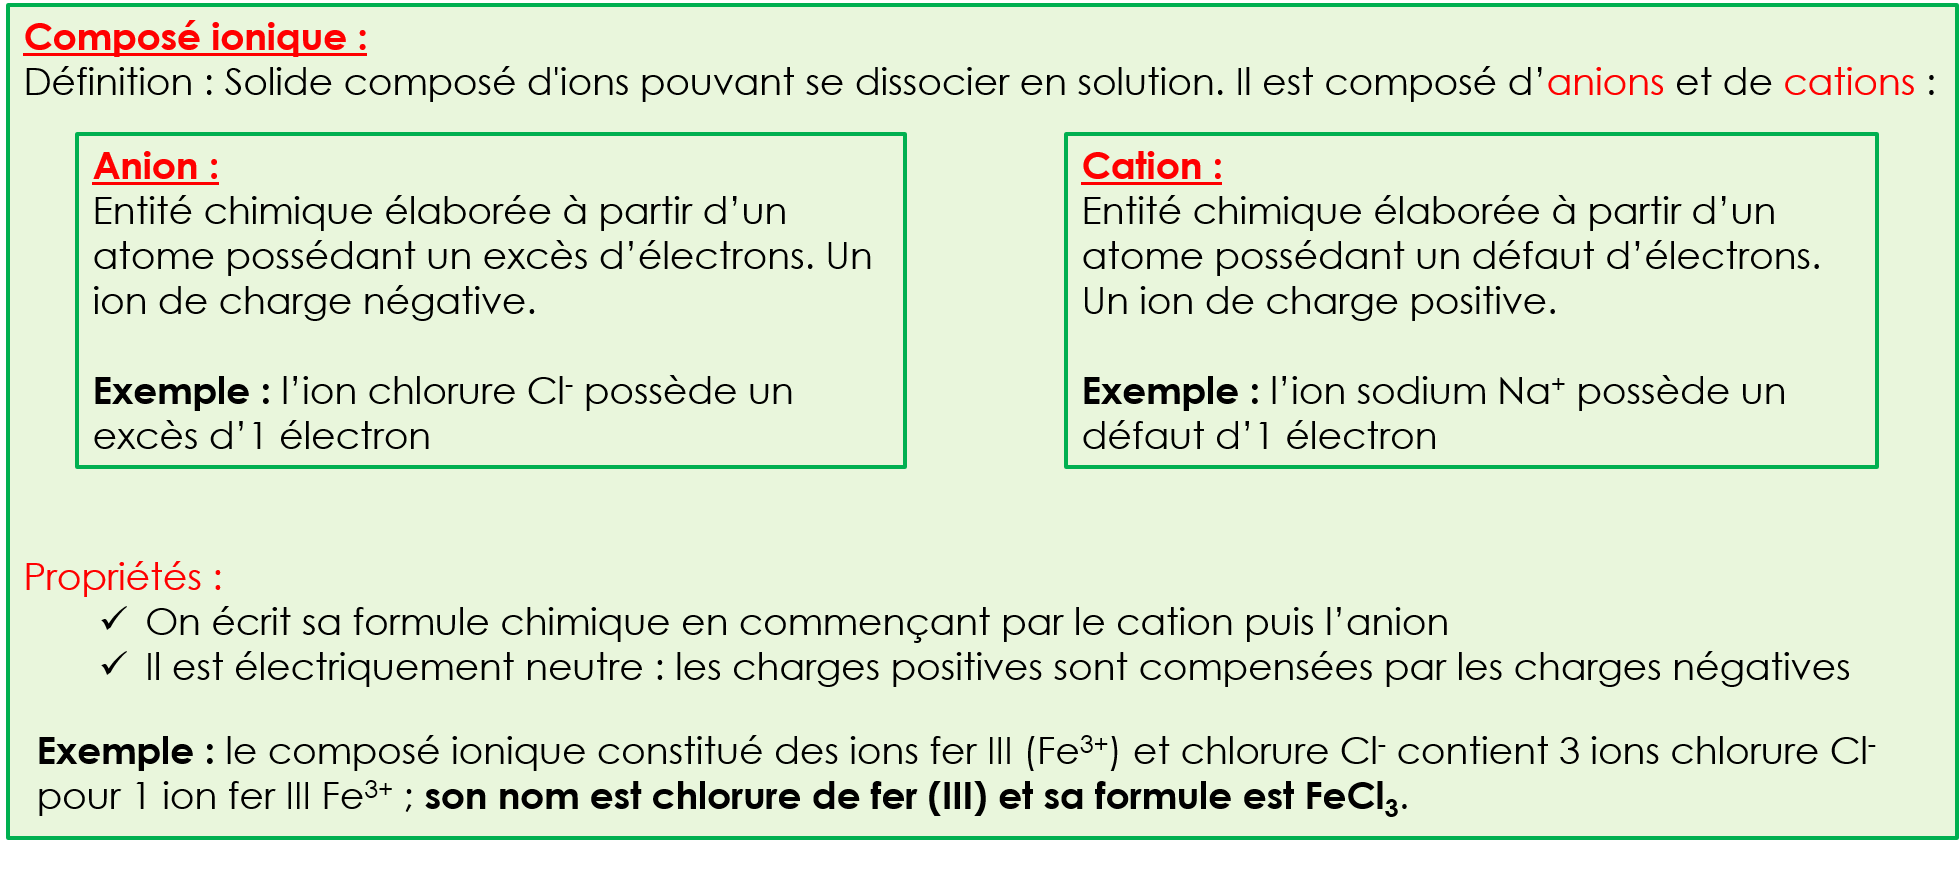
\includegraphics[scale=0.55]{Images/Solide_ionique.png}
\end{center}
\end{doc}

\question{Rappeler la problématique et proposer une hypothèse sur la nature des ions constituants le nigari.}{~}{0}
%\\
\question{Proposer un protocole expérimental permettant d’identifier les ions présents dans le Nigari. Vous pourrez utiliser des schémas accompagnés de phrases explicatives.}{~}{0}

\begin{center}
\begin{mdframed}[style=titr, leftmargin=60pt, rightmargin=60pt, innertopmargin=7pt, innerbottommargin=7pt, innerrightmargin=8pt, innerleftmargin=8pt]

\begin{center}
\begin{Large}
    \textcolor{red}{Appeler le professeur pour vérifier votre protocole.}
\end{Large}
\end{center}
\end{mdframed}
\end{center}

%\\
\question{Mettre en œuvre le protocole expérimental précédent.}{}{0}
%\\
\question{Noter vos observations.}{~}{0}
%\\
\question{Interprétations : en déduire les ions présents dans le nigari.}{~}{0}
%\\
\question{Conclusion : à l'aide du document 3, en déduire le nom et la formule du composé ionique constituant le nigari. Indiquer les effets bénéfiques et applications du nigari.}{~}{0}
\newpage

\begin{difficile}{Bilan à retenir}
\vspace{0.5cm}
\begin{multicols}{2}
\begin{center}
    On aurait pu tout faire à l'aide de ce logiciel de simulation (merci l'université du Colorado !) :

    \url{https://phet.colorado.edu/fr/simulations/geometric-optics-basics}\\
    \vspace{4cm}
    \begin{Large}
        \textbf{Mais c'est quand même bien mieux d'expérimenter en TP, non ??}
    \end{Large}
\end{center}

%\begin{center}
 %   \includegraphics[scale=0.15]{Images/Joyeux_noel_dispersé.png}
%\end{center}
\end{multicols}


\end{difficile}
%\newpage
%\papiermillimetre